\documentclass[UTF8]{ctexart}
\usepackage{subfigure}
\usepackage{caption}
\usepackage{amsmath}
\usepackage{amssymb}
\usepackage{pifont}
\usepackage{geometry}
\usepackage{graphicx}
\usepackage{gensymb}
\usepackage{wrapfig}
\usepackage{titlesec}
\usepackage{float}
\usepackage{diagbox}
\usepackage{fancyhdr}
\usepackage{color}
\pagestyle{plain}
\geometry{a4paper,scale=0.8}
\CTEXsetup[format+={\raggedright}]{section} 
\title{通网2016期中}
\author{Deschain}
\titlespacing*{\section}
{0pt}{0pt}{0pt}
\titlespacing*{\subsection}
{0pt}{0pt}{0pt}
\titlespacing*{\paragraph}
{0pt}{0pt}{0pt}
\titlespacing*{\subparagraph}
{0pt}{0pt}{0pt}
\titleformat*{\section}{\normalsize}
\begin{document}
\maketitle
\section*{1.}
抛掷硬币的试验,从每一组试验均为掷至第一次出现正面即停止。将这一组所需掷硬币的次数记下来。如果
需要做10000组这样的试验,试验记录至少需要多少比特,或平均到每一组需要记多少个比特?
\section*{2.}
随机变量X,Y均取值于\{0,1\},组合XY取值00,01,10,11的概率分别为$\frac{1}{3},
  \frac{1}{3},0,\frac{1}{3}$。随机变量$Z=X+Ymod2$。求:\\
(1)$H(X),H(Y)$\\
(2)$H(X\lvert Y),H(Y\lvert X),I(X,Y)$\\
(3)$H(X\lvert Z),H(XYZ)$\\
\section*{3.基本概念题\\}
相同带宽B情况下,以下传输方式可达到最高的传输比特率由高到低排序(并用大于号">"或等于号"="相连,
各自最高可达比特率的情况):2ASK,BPSK,正交2FSK,QPSK,4ASK,正交4FSK,16QAM,16ASK,正交16FSK。
\section*{4.}
不归零方波双极性传输中,信号电平为+A和-A,成形滤波器响应在$[0,\frac{2}{3}T_s]$
内为1,其他时间为0,其中$T_s$为符号间隔,发送+A的概率为$\frac{2}{3}$,发送-A的概率为$\frac
  {1}{3}$,不同符号的发送电平之间独立。\\
(1)写出它的匹配滤波器冲激响应表达式,并画图;\\
(2)画出发送信号的功率谱密度示意图,标出关键频率的位置(如能写出功率谱表达式,依正确程度可不同
程度加分);\\
(3)画出单个符号传输时(假设发送电平-A)匹配滤波器输出的波形,标出最佳采样点位置及其幅度;\\
(4)当采样点噪声功率为$\sigma^2$时,给出最佳判决门限。\\
(5)写出误符号率最低时的误符号率公式与$\frac{E_s}{n_0}$的关系。\\
(6)写出误比特率最低时的误比特率公式与$\frac{E_b}{n_0}$的关系(附加题)。\\
\section*{5.系统设计题\\}
\begin{figure}[H]
  \centering
  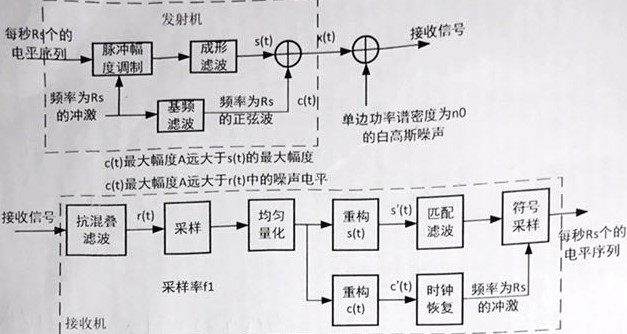
\includegraphics[width=15cm,height=8cm]{5.jpg}
\end{figure}
某通信系统,发射机和信道(AWGN)如上图上部所示,为了在收段便于恢复定时时钟,这里将本地符号时钟以
正弦波的形式通过信道传递给了收段。\\
$\quad\quad$接收端为了便于处理,先对接收波形进行了数字化,再对数字化以后的波形,分别重构出信号分量(
含带内噪声)和定时脉冲。这样,发射机、信道、接收机就构成了一个输入电平序列、输出电平序列出的等效
信道。\\
$\quad\quad$为了在接收端符号采样点信号分量无失真,采用了滚降系数为$\alpha=0.5$的升余弦滤波(总频响)
,抗混叠滤波器为带内平坦的理想低通滤波器。\\
$\quad\quad$假设发送信号中的信号分量$s(t)$功率为$P$,假设电平换算功率时的阻抗为1欧姆,$c(t)$最大幅度
为A,信道单边噪声功率谱密度为$n_0$,输入电平序列速率为每秒$R_s$个电平,接收机对接收波形数字化时
采用的时域均匀采样,采样率为$f_1$,量化器的量化电平数为$Q$(远大于1)。\\
回答以下问题(如果有些步骤走不下去,可以先假设已经能得到某些中间结果,用一个符号来表示,继续走下
去):\\
(1)如果希望接收机输出符号采样点信噪比最大,需合理设计接收匹配滤波器和发送成型滤波,请画出此时的
匹配滤波器频谱(幅度谱),以及$x(t)$的功率谱(只要大致形状,标出关键频率点的值)。\\
(2)为了能在无噪声情况下正确恢复$s(t)$和$c(t)$,需要的接收机量化前的采样率$f_1$最低为多少,给
出考虑因素。\\
(3)为什么需要抗混叠滤波,在采样率$f_1$最低的情况下,该抗混叠滤波器截止频率该取多少?\\
(4)采样Q电平量化后(Q远大于1),求重构波形$s(t)$的信噪比(注意含信道噪声和量化噪声,要求其中的
$s(t)$信号部分分量无失真)的表达式。\\
(5)最终符号采样点信噪比的表达式(假设符号采样定时已被准确修复。)\\
(6)当采用M电平(均匀间隔,关于0对称)传输时,求误符号率表达式。\\
(7)当不限电平数及其概率分布的情况下,该收发系统可以传输的信号速率最大可以达到多少,此时的输入电
平应呈现什么分布?\\
\end{document}